% ------------------------------------------------------------------------------
% TYPO3 CMS 7.2 - What's New (English Version)
%
% @author	Michael Schams <schams.net>
% @license	Creative Commons BY-NC-SA 3.0
% @link		http://typo3.org/download/release-notes/whats-new/
% @language	English
% ------------------------------------------------------------------------------
% LTXE-CHAPTER-UID:		93899f32-8efb477e-ed6973d2-b679bd8e
% LTXE-CHAPTER-NAME:	Backend User Interface
% ------------------------------------------------------------------------------

\section{Administratorski interfejs}
\begin{frame}[fragile]
	\frametitle{Administratorski interfejs}

	\begin{center}\huge{Poglavlje 1:}\end{center}
	\begin{center}\huge{\color{typo3darkgrey}\textbf{Administratorski interfejs}}\end{center}

\end{frame}

% ------------------------------------------------------------------------------
% LTXE-SLIDE-START
% LTXE-SLIDE-UID:		d668952b-ffeb36a1-ab2a6d4a-373810d0
% LTXE-SLIDE-ORIGIN:	c151f95c-3fe3eb42-442ce244-5f987f80 English
% LTXE-SLIDE-TITLE:		Customized BE login form
% LTXE-SLIDE-REFERENCE:	unknown
% ------------------------------------------------------------------------------
\begin{frame}[fragile]
	\frametitle{Administratorski interfejs}
	\framesubtitle{Prilagodljiva forma za prijavljivanje}

	Sistemsko prosirenje administratorskog interfejsa dozvoljava podesavanje i postavljanje slike, logoa i boje na formu za prijavljivanje

	\begin{figure}
		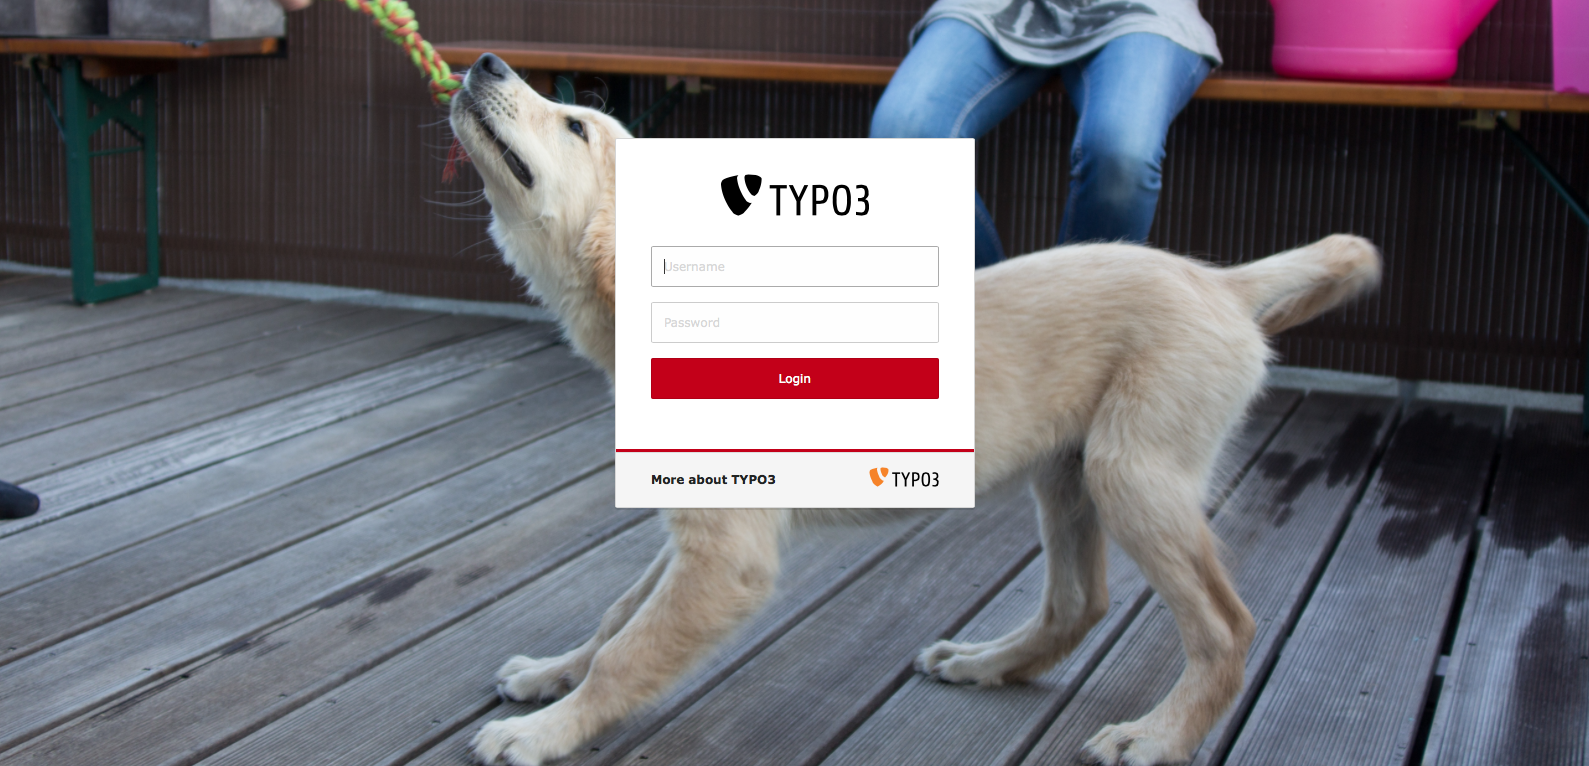
\includegraphics[width=0.75\linewidth]{BackendUserInterface/Login.png}
	\end{figure}

\end{frame}

% ------------------------------------------------------------------------------
% LTXE-SLIDE-START
% LTXE-SLIDE-UID:		20da3bb0-c12c5d59-19b1cec9-74d3df8a
% LTXE-SLIDE-ORIGIN:	e2e353ae-3b2b5c00-0cd7c57d-d97d22c9 English
% LTXE-SLIDE-TITLE:		Add image cropping
% LTXE-SLIDE-REFERENCE:	Feature-65584-AddImageCropping.rst
% ------------------------------------------------------------------------------
\begin{frame}[fragile]
	\frametitle{Administratorski interfejs}
	\framesubtitle{Manipulisanje slikom: Secenje}

	Nova funkcionalnost za manipulisanje nad slikom dozvoljava uredniku da sece slike u samom administratorskom interfejsu.
	Ova opcija mora biti posebno ukljucena ("Exclude Fields"):

	\begin{figure}
		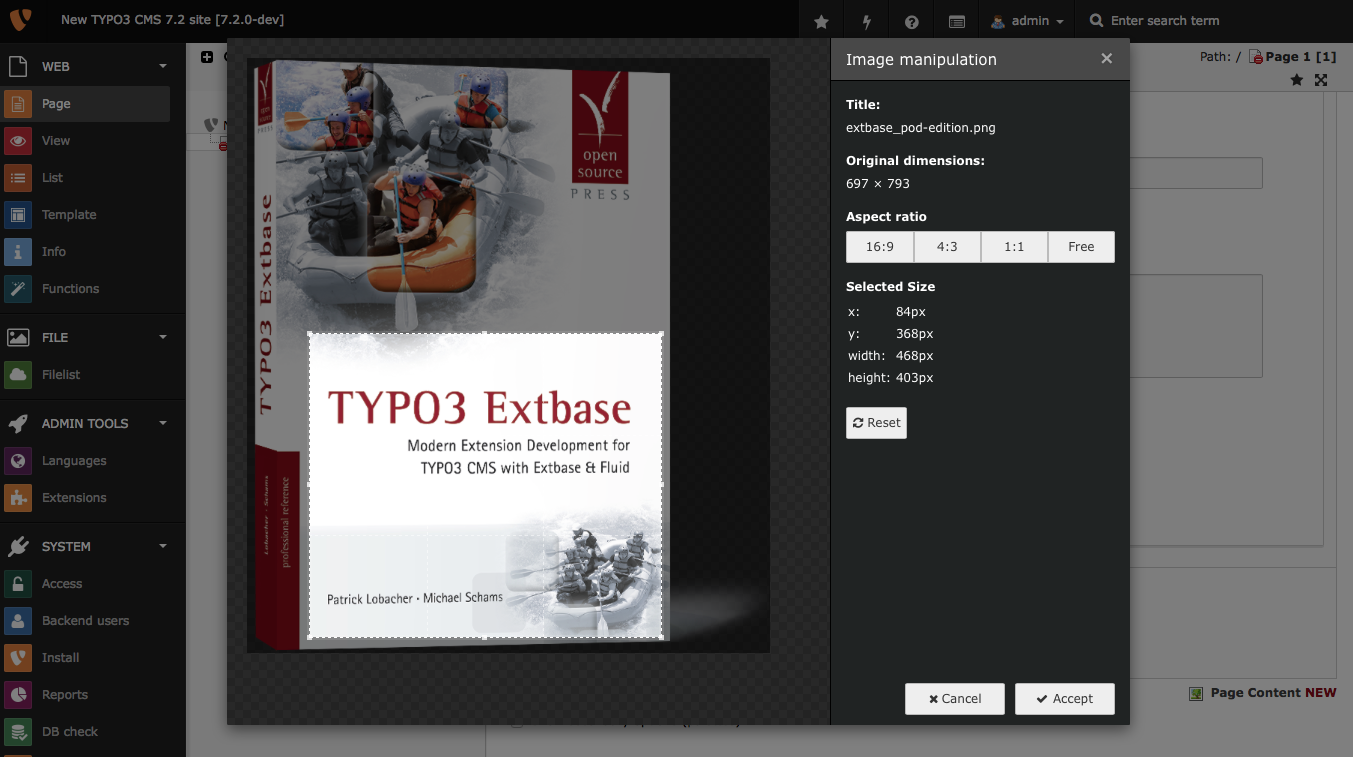
\includegraphics[width=0.7\linewidth]{BackendUserInterface/ImageCropping.png}
	\end{figure}

\end{frame}

% ------------------------------------------------------------------------------
% LTXE-SLIDE-START
% LTXE-SLIDE-UID:		0ff7f3f4-b90c4c88-c900bdf8-b5ed7e0d
% LTXE-SLIDE-ORIGIN:	301dfea9-d2debf3e-dcaa7bcd-205e5990 English
% LTXE-SLIDE-TITLE:		Add backend user groups to backend user module
% LTXE-SLIDE-REFERENCE:	Feature-64686-AddBackendUserGroupsToBackendUserModule.rst
% ------------------------------------------------------------------------------
\begin{frame}[fragile]
	\frametitle{Administratorski interfejs}
	\framesubtitle{Administratorske grupe}

	Administratorske grupe se sada mogu odrzavati i pregledavati u podmodulu "Backend Users" modula:

	\begin{figure}
		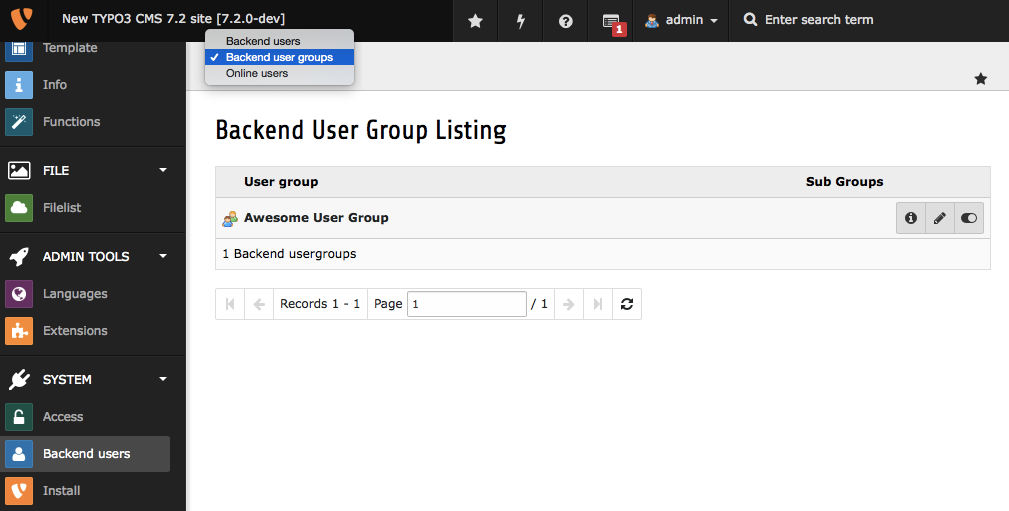
\includegraphics[width=0.70\linewidth]{BackendUserInterface/UserGroups.png}
	\end{figure}

\end{frame}

% ------------------------------------------------------------------------------
% LTXE-SLIDE-START
% LTXE-SLIDE-UID:		30fae622-2214ec24-d6d5fcdb-b288fda2
% LTXE-SLIDE-ORIGIN:	daa83c1e-08d2716b-de74cbda-42361551 English
% LTXE-SLIDE-TITLE:		Extension Manager: Disable automatic installation
% LTXE-SLIDE-REFERENCE:	Feature-50501-DisableAutomaticExtInstallation.rst
% ------------------------------------------------------------------------------
\begin{frame}[fragile]
	\frametitle{Administratorski interfejs}
	\framesubtitle{Onesposobiti automatsku instalaciju prosirenja}

	Administratori sada mogu konfigurisati Extension Manager tako da preuzeta prosirenja ne instalira odmah:

	\begin{figure}
		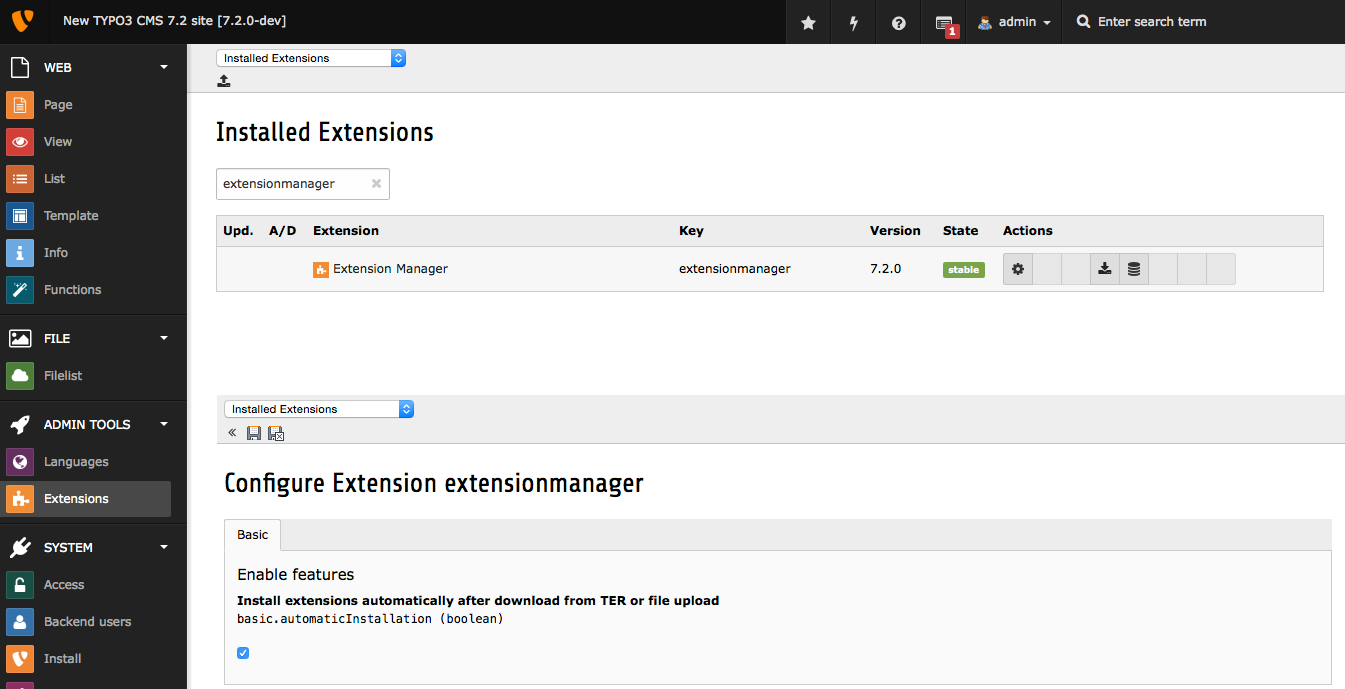
\includegraphics[width=0.70\linewidth]{BackendUserInterface/ExtManager.png}
	\end{figure}

\end{frame}

% ------------------------------------------------------------------------------
% LTXE-SLIDE-START
% LTXE-SLIDE-UID:		eb529634-6a188890-6e5cdce5-c4ec4ab4
% LTXE-SLIDE-ORIGIN:	20769920-da9df227-c3b527b9-9a23bac1 English
% LTXE-SLIDE-TITLE:		Show remaining characters below text fields
% LTXE-SLIDE-REFERENCE:	Feature-66029-ShowRemainingCharactersBelowTextFields.rst
% ------------------------------------------------------------------------------
\begin{frame}[fragile]
	\frametitle{Administratorski interfejs}
	\framesubtitle{Broj preostalih karaktera kod tekstualnih polja}

	Broj preostalih karaktera prikazan je ispod tekstualnih polja:

	\begin{figure}
		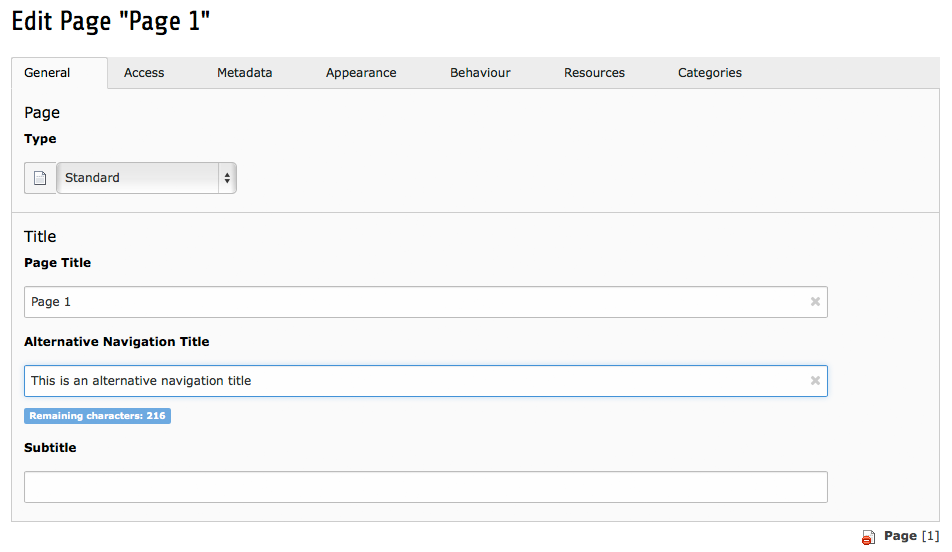
\includegraphics[width=0.70\linewidth]{BackendUserInterface/RemainingCharacters.png}
	\end{figure}

\end{frame}

% ------------------------------------------------------------------------------
% LTXE-SLIDE-START
% LTXE-SLIDE-UID:		ef18237a-4199d95d-c6f3a6e6-9b5462bd
% LTXE-SLIDE-ORIGIN:	ff760b86-9d6b1ecd-d0e98565-f23c51f0 English
% LTXE-SLIDE-TITLE:		Show confirm message on closing an editform with unsaved changes
% LTXE-SLIDE-REFERENCE:	Feature-65996-AddConfirmationOnCloseEditformWithUnsavedChanges.rst
% ------------------------------------------------------------------------------
\begin{frame}[fragile]
	\frametitle{Administratorski interfejs}
	\framesubtitle{Potvrda o nesacuvanim promenama}

	Novi prozor za potvrdu upozorava urednike da ce izgubiti nesacuvane promene:

	\begin{figure}
		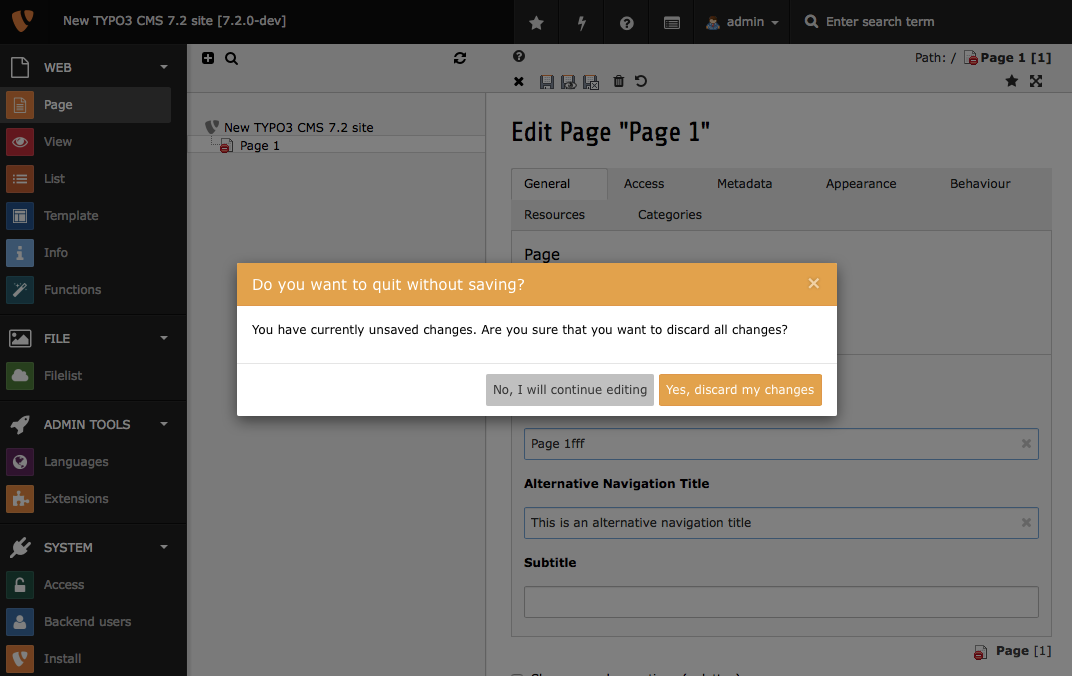
\includegraphics[width=0.65\linewidth]{BackendUserInterface/ClosingDialog.png}
	\end{figure}

\end{frame}

% ------------------------------------------------------------------------------
% LTXE-SLIDE-START
% LTXE-SLIDE-UID:		6c961145-469a7b12-7ce9ecf0-e0a74315
% LTXE-SLIDE-ORIGIN:	6ac9a35e-46541895-7509263e-28fb799f English
% LTXE-SLIDE-TITLE:		System Information Dropdown
% LTXE-SLIDE-REFERENCE:	Feature-65767-SystemInformationDropdown.rst
% ------------------------------------------------------------------------------
\begin{frame}[fragile]
	\frametitle{Administratorski interfejs}
	\framesubtitle{Sistemske informacije u padajucem meniju}

	Padajuci meni pokazuje nekoliko informacija o sistemu na koji je TYPO3 instaliran.
	Ovi podaci se mozgu prosiriti:\newline
	\small(za dodatne informacije pogledati poglavlje "Korenite promene")\normalsize

	\begin{figure}
		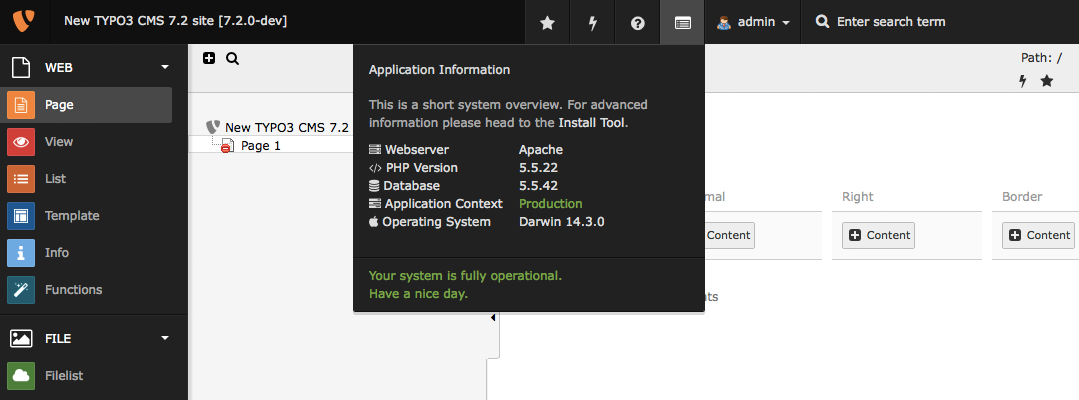
\includegraphics[width=0.85\linewidth]{BackendUserInterface/SystemInformation.png}
	\end{figure}

\end{frame}

% ------------------------------------------------------------------------------
% LTXE-SLIDE-START
% LTXE-SLIDE-UID:		920f1ad5-d662f6a9-b6c5a660-891ed972
% LTXE-SLIDE-ORIGIN:	79a2ee0c-3439d600-08990adb-6bed8c19 English
% LTXE-SLIDE-TITLE:		Ask for old password when changing
% LTXE-SLIDE-REFERENCE:	commit bf6f5226eb6cb441bb53657a88ef42f1cdb5155f
% ------------------------------------------------------------------------------
\begin{frame}[fragile]
	\frametitle{Administratorski interfejs}
	\framesubtitle{Promena sifre}

	Administratori i editori moraju ukucati trenutnu (staru) sifru kako bi je promenili u novu:

	\begin{figure}
		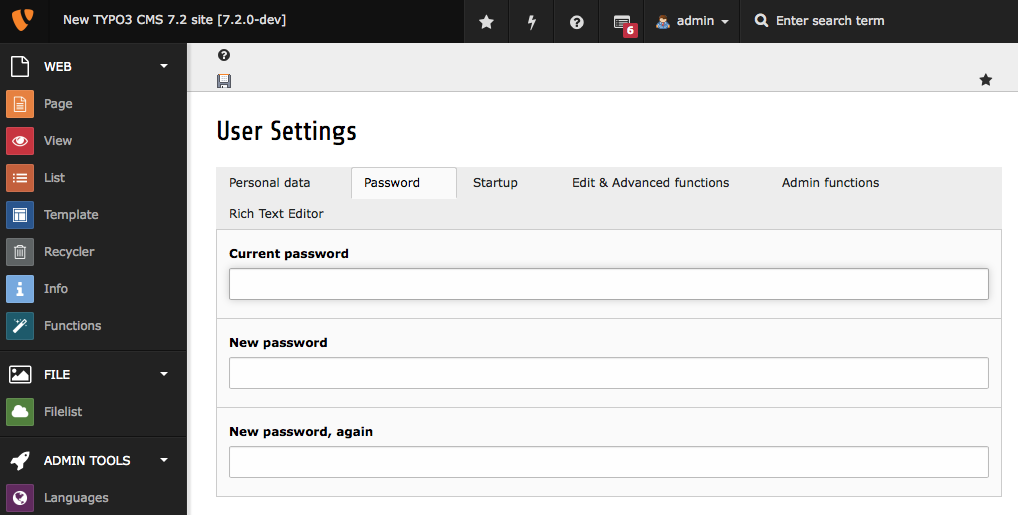
\includegraphics[width=0.7\linewidth]{BackendUserInterface/Password.png}
	\end{figure}

\end{frame}

% ------------------------------------------------------------------------------
% LTXE-SLIDE-START
% LTXE-SLIDE-UID:		c41f4ab4-d60ea90f-6f7205a0-b36629a2
% LTXE-SLIDE-ORIGIN:	7725bce9-e606f055-bf2e7b4a-e870fe2a English
% LTXE-SLIDE-TITLE:		Add icon for "Show Content From Page"
% LTXE-SLIDE-REFERENCE:	commit f8aa3eea9aed97a901ef0c3e7c650e1218839596
% ------------------------------------------------------------------------------
\begin{frame}[fragile]
	\frametitle{Administratorski interfejs}
	\framesubtitle{Ikonica za "Show Content from Page"}

	Nova ikonica u stablu strana oznacava da koja strana prikazuje sadrzaj sa neke druge strane:

	\begin{figure}
		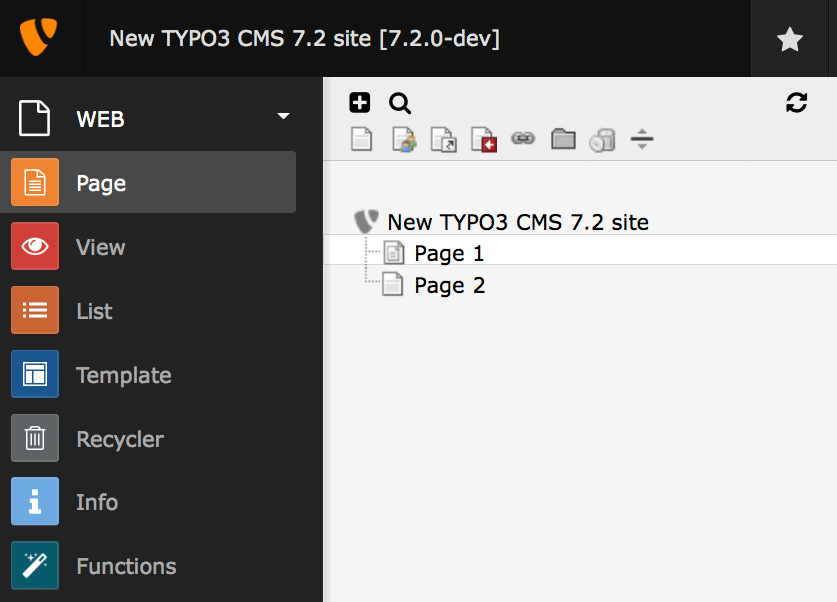
\includegraphics[width=0.45\linewidth]{BackendUserInterface/ShowContent.png}
	\end{figure}

\end{frame}

% ------------------------------------------------------------------------------
% LTXE-SLIDE-START
% LTXE-SLIDE-UID:		d9d31f24-b0d16cf8-941d1605-f247e598
% LTXE-SLIDE-ORIGIN:	5ac2de45-9be12bf9-1c326192-602839fb English
% LTXE-SLIDE-TITLE:		Extension Manager: Choose version for update
% LTXE-SLIDE-REFERENCE:	commit a26396a4530b530744ec8b36c5fb5606789a6739
% ------------------------------------------------------------------------------
\begin{frame}[fragile]
	\frametitle{Administratorski interfejs}
	\framesubtitle{Nadogradnja prosirenja}

	Kada se nadogradjuje prosirenje sada je moguce izabrati zeljenu verziju:

	\begin{figure}
		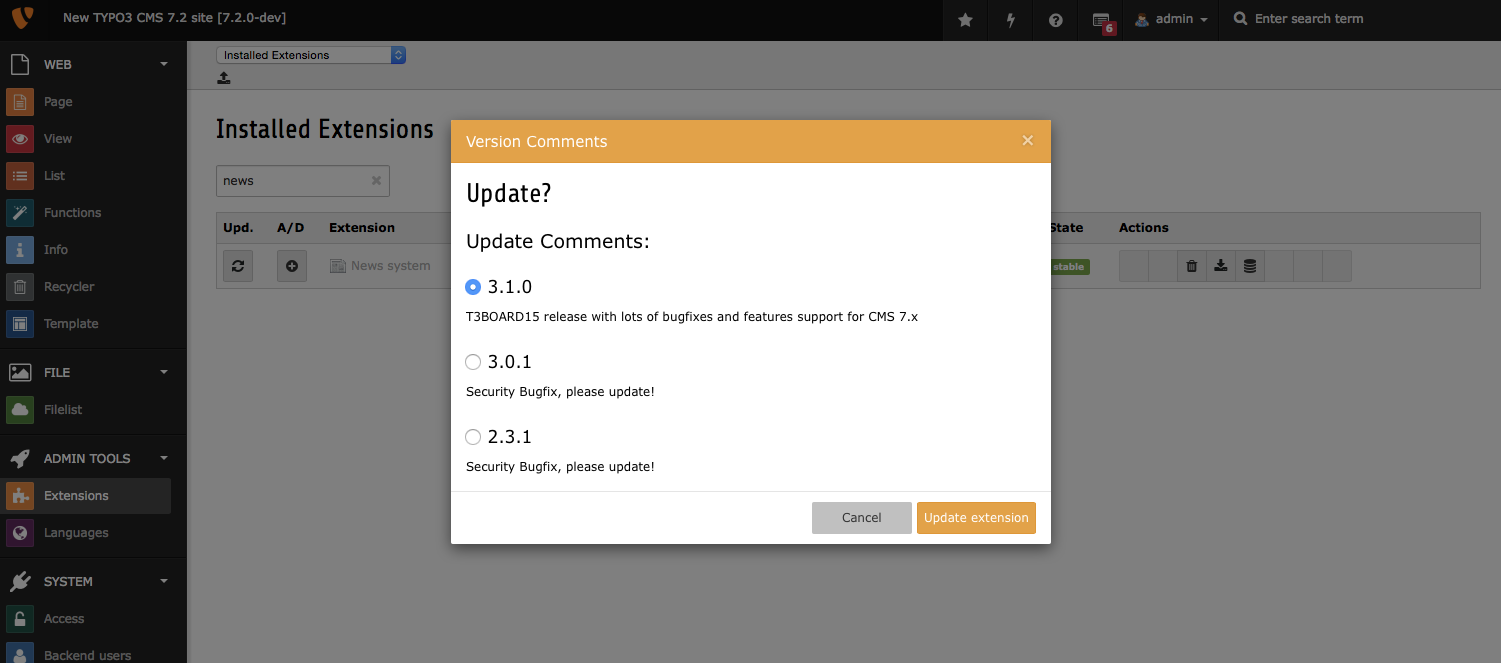
\includegraphics[width=0.75\linewidth]{BackendUserInterface/Update.png}
	\end{figure}

\end{frame}

% ------------------------------------------------------------------------------
% LTXE-SLIDE-START
% LTXE-SLIDE-UID:		442157d1-fc28dbf4-3982777d-b10f1f3b
% LTXE-SLIDE-ORIGIN:	f6be31f7-155d676c-0e551545-3fc89e89 English
% LTXE-SLIDE-TITLE:		Add scheduler task to remove deleted records
% LTXE-SLIDE-REFERENCE:	Feature-32651-AddSchedulerTaskToRemoveDeletedRecords.rst
% ------------------------------------------------------------------------------
\begin{frame}[fragile]
	\frametitle{Administratorski interfejs}
	\framesubtitle{Recycler Task}

	Novi scheduler task za sistemsko prosirenje \texttt{recycler} uklanja obrisane rekorde iz kontent tabela u bazi podataka. Maksimalan vremenski raspon izmedju brisanja kao i zahvacene tabele mogu se konfigurisati u instrukciji.
	\newline
	Ovo se takodje moze odnositi i na fajlove ukoliko su referencirani u elementu sadrzaja.

	\begin{figure}
		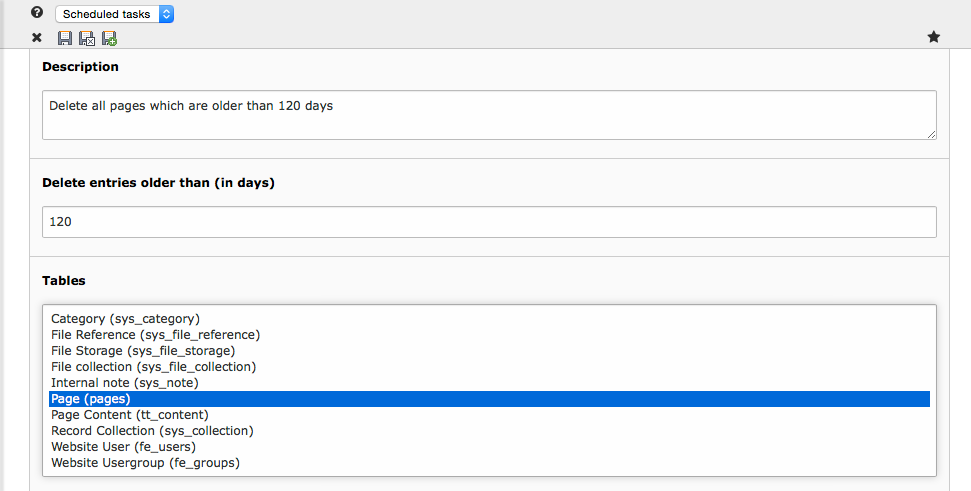
\includegraphics[width=0.68\linewidth]{BackendUserInterface/RecyclerTask.png}
	\end{figure}

\end{frame}

% ------------------------------------------------------------------------------
